\section{Requirements}
\label{sec:Requirements}

\subsection{Overview}
\label{sec:Requirements>Overview}
Initially, this project was conceived by Dr. Kenny Hunt, who served as the advisor, and he gave almost all of the requirements in an introductory meeting. Both the advisor, who is also the project sponsor, and the developer, who is also the author, are the stakeholders of the project.

After that, the advisor met with the developer every week to gather informal functional requirements of this project, and he would also refine any previous requirements that were given. These requirements played a crucial role in the development of the map generator. On the one hand, the scope of development was clarified, and on the other hand, the necessary algorithms were compiled to maintain the continuation of development.

\subsection{Functional Requirements}
\label{sec:Requirements>Functional Requirements}
There are two roles for this system: ``admins'' and ``users''. As a result, the following functional requirements were established for the project:
\begin{enumerate}
  \item As an admin or a user, I need to be able to:
  \begin{enumerate}
    \item Log in with a unique email and password
    \item Log out with the ended session
    \item Edit personal profile by changing email, first name, last name, and password
  \end{enumerate}
  \item As an admin, I want to be able to:
  \begin{enumerate}
    \item View all users
    \item Enable or disable users
    \item Search for users using any combination of email, first name, and last name
  \end{enumerate}
  \item As a user, I want to be able to:
  \begin{enumerate}
    \item Sign up with a unique email, first name, last name, long password, and confirmed password
    \item View all of the maps that I have created
    \item View all maps shared with me
    \item Search for maps using any combination of the map name, created date, edited date, the owner's email, the owner's first name, and the owner's last name
    \item Download viewable maps in PNG or SVG format
    \item Make maps public or private
    \item Create maps with a name
    \item Delete maps
    \item Edit maps
  \end{enumerate}
\end{enumerate}

Figure \ref{fig:Use Case Diagram} is the Use Case Diagram that describes the functionalities to be implemented by this web application.

\begin{figure}[!htbp]
\centering
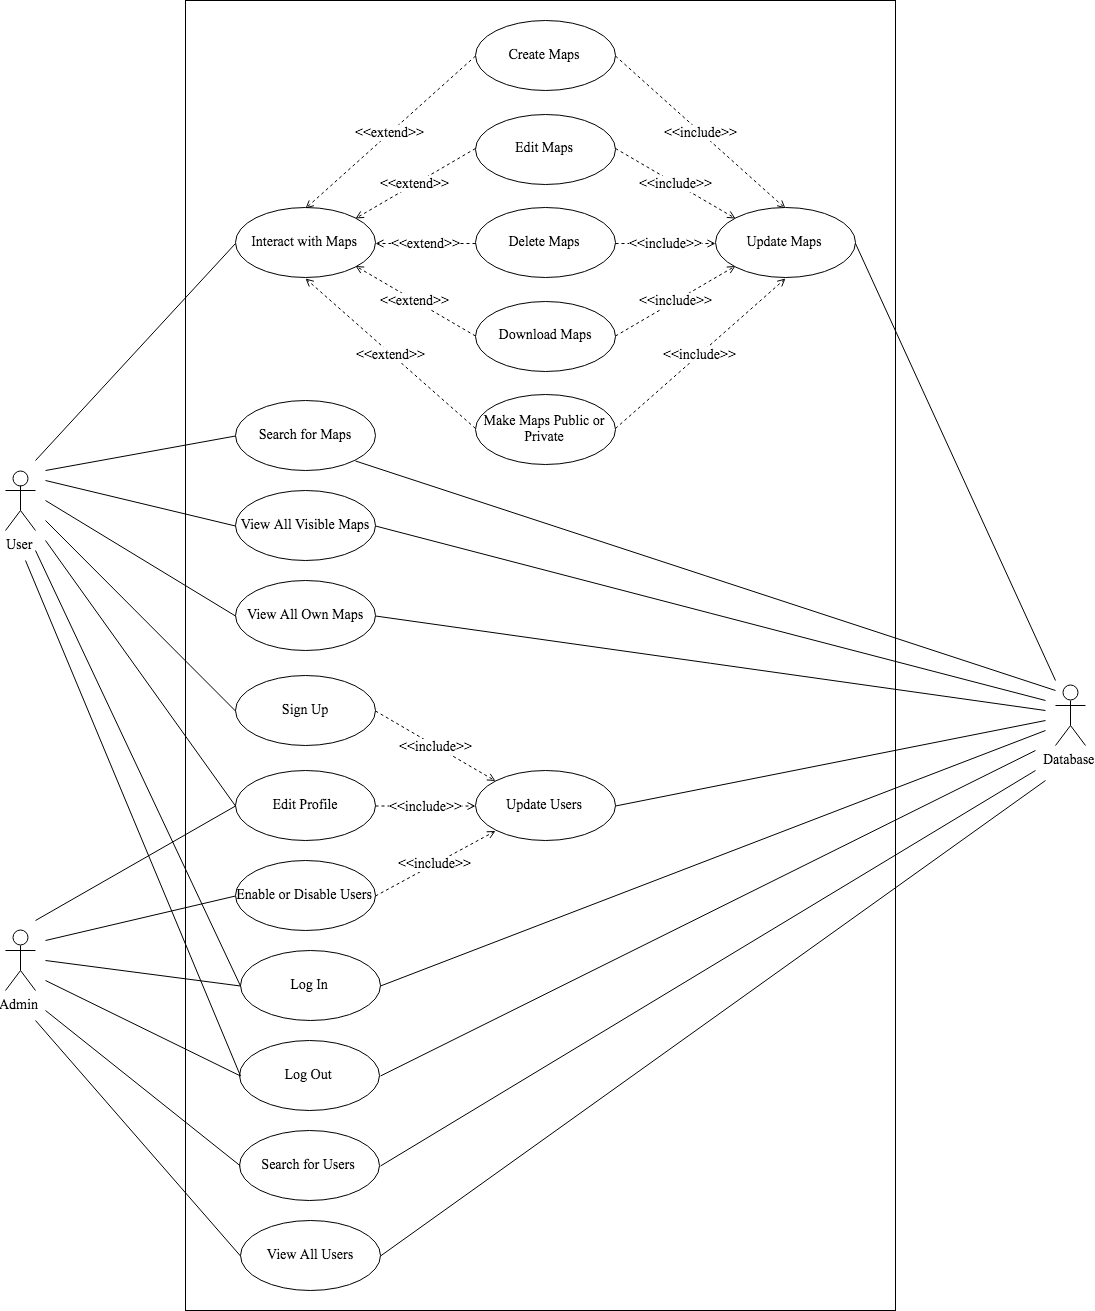
\includegraphics[width=\textwidth]{section02/assets/use_case.png}
\caption[Use Case Diagram]{\label{fig:Use Case Diagram}Use Case Diagram}
\end{figure}

\subsection{Non-Functional Requirements}
\label{sec:Requirements>Non-Functional Requirements}
There are numerous non-functional requirements for this system: response time, availability, usability, security (authentication, authorization, integrity, privacy, etc.), and so on. For this application, we focused on the following requirements:
\begin{enumerate}
  \item Security:
  \begin{enumerate}
    \item Input Validation:
    \begin{enumerate}
      \item Add validations at both client and server sides
      \item All methods should always validate all parameters in the server-side
    \end{enumerate}
    \item Password Encryption:
    \begin{enumerate}
      \item Shall always be encrypted
      \item Not even the system administrators shall see clear text passwords
      \item Applying a hashing algorithm to passwords
    \end{enumerate}
    \item Prohibiting Cross Site Scripting (XSS):
    \begin{enumerate}
      \item Never insert data anywhere in a ``script'' element
      \item Never insert data in an HTML comment
      \item Never insert data anywhere in CSS
      \item Never insert data in an attribute name
      \item Never insert data in an attribute value
      \item Never insert data in a tag name
    \end{enumerate}
    \item Secure Session Cookie:
    \begin{enumerate}
      \item Set the ``Secure'' cookie attribute and instruct web browsers to send the cookie only over encrypted, e.g., HTTPS, links.
      \item Set the ``HttpOnly'' attribute true and prohibiting the JavaScript code from reading the cookie via the DOM ``document.cookie'' JavaScript object.
      \item Always change the session id after login
    \end{enumerate}
  \end{enumerate}
  \item Performance:
  \begin{enumerate}
    \item High performance of rendering map:
    \begin{enumerate}
      \item Compare and select the most appropriate and the fastest way to render maps, e.g., canvas, SVG
    \end{enumerate}
  \end{enumerate}
\end{enumerate}

\subsection{Selection of Software Development Life Cycle Model}
\label{sec:Requirements>SDLC}
We analyzed and summarized the following possible risks:
\begin{enumerate}
  \item Lack of experience developing in a map generation
  \item The certainty whether a third-party library was available as the map rendering engine
  \item The potential misunderstanding between the advisor and the developer with respect to the requirements
\end{enumerate}

To reduce or avoid these risks, two life cycle models were considered: waterfall and agile. Because of our development model is flexible and the frequent communication between the sponsor and the developer, the waterfall model, is beyond our consideration. Unlike the waterfall model, we only need initial planning to start this project, and every time the new requirements are almost based on the previous one. Finally, the agile model was chosen, which is shown in Figure \ref{fig:Agile Model}.

\begin{figure}[htb]
\centering
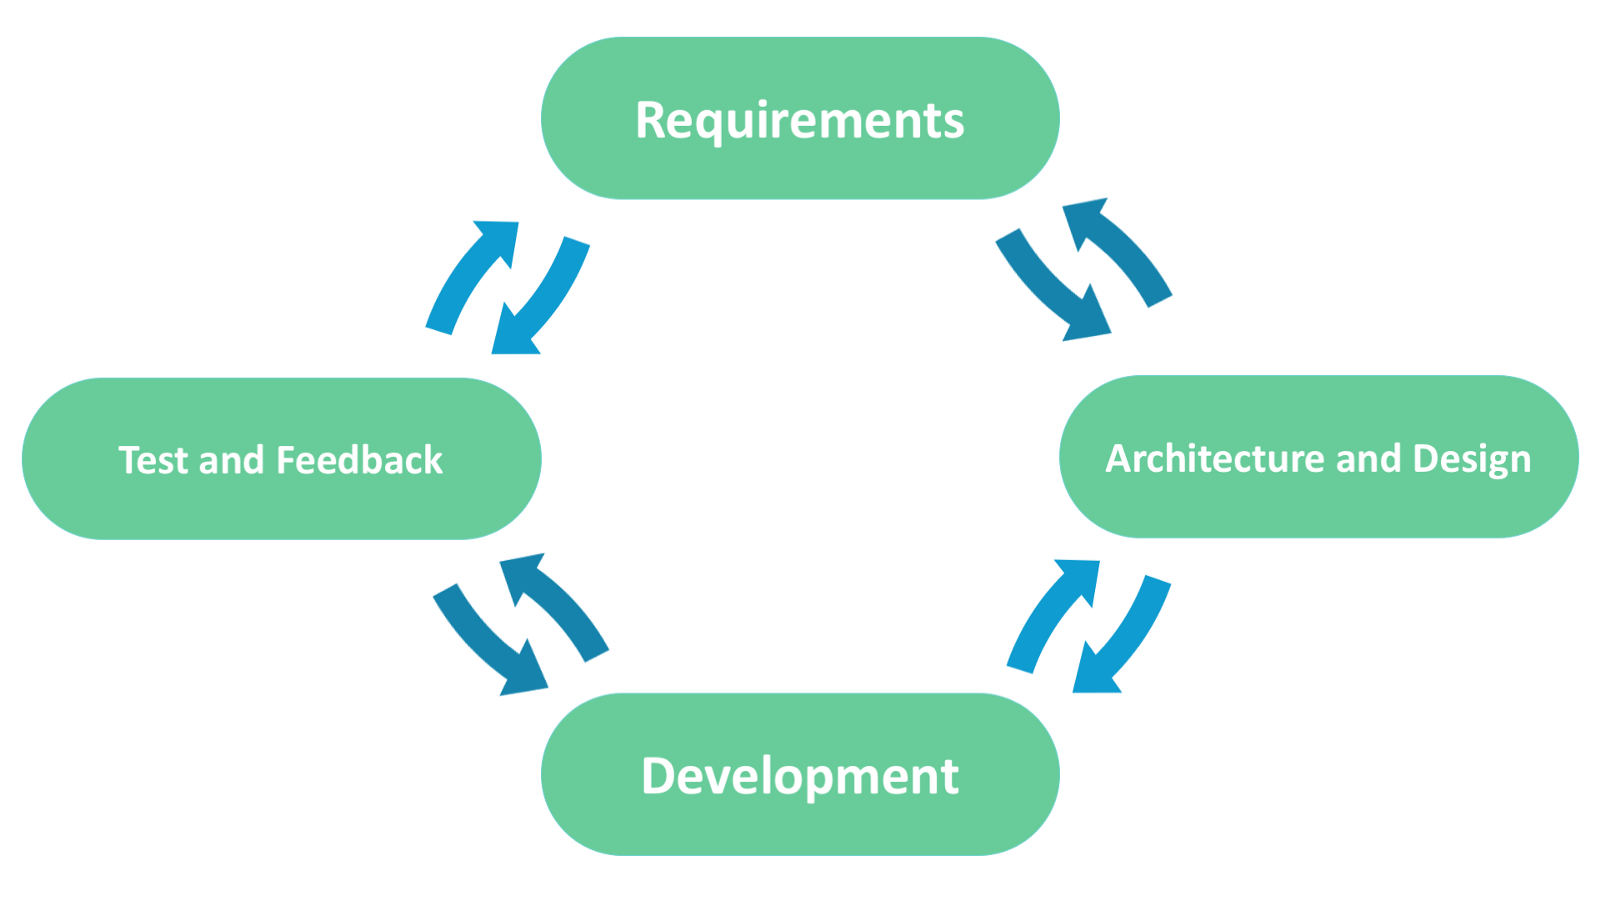
\includegraphics[width=\textwidth]{section02/assets/agile.png}
\caption[Agile Development Life Cycle Model]{\label{fig:Agile Model}Agile Development Life Cycle Model}
\end{figure}

An agile methodology is a practice that helps continuous iterations of development and testing in the software development process. In this model, development and testing activities are concurrent. Furthermore, the agile model is a combination of iterative and incremental process models, which breaks the product into small incremental builds. These builds are provided in iterations. Each iteration typically lasts from about one to three weeks.

At the end of each iteration, a working product demo is displayed to stakeholders. There are several known advantages and disadvantages of using the agile model in this project:
\begin{enumerate}

  \item Advantages:
  \begin{enumerate}
    \item Easy to manage
    \item Little or no planning required
    \item Gives flexibility to developers
    \item Resource requirements are minimum
    \item Suitable for fixed or changing requirements
  \end{enumerate}

  \item Disadvantages:
  \begin{enumerate}
    \item More risks of sustainability, maintainability, and extensibility
    \item An overall plan, an agile leader (the advisor) is a must without which it will not work
    \item There is a very high individual dependency since there is minimum documentation generated
  \end{enumerate}

\end{enumerate}
